\section{3D-Laplace}
The previous sub-section described the use of 2-dimensional noise on geographical data.
This approach has recently been extended to support 3-dimensional data, which benefits indoor navigation \citep{9646489}.
The method is similar to the 2D approach but includes the azimuth angle $\psi$ besides the polar angle $\theta$ and radial distance $r$.

\subsection{Geo-indistinguishability}
To establish the same privacy guarantees for 3-dimensional data as for 2-dimensional data, the original equation \ref{algo:2d-geo-indistinguishability} is extended \citep{9646489}.
\begin{equation}
  K(x_1)(z) \le e^{\epsilon * d_3(x_1, x_2)} K(x_2)(z)
  \label{algo:3d-geo-indistinguishability}
\end{equation}
Where $x_1$ and $x_2$ are two real data points in the same dataset $X$.
%The more $x_1$ and $x_2$ are similar, the more the perturbed location distributions $K(x_1)(z)$ and $K(x_2)(z)$ need to be similar.
\subsection{Spherical Laplace}
The implementation of Min et al. projects the dimensions onto a sphere instead of a circle \citep{9646489}.
This sphere is a unit sphere calculated with a radius of 1.
The polar angle $\theta$ and azimuth angle $\psi$ are randomly calculated based on this sphere. \newline
\textbf{Calculating $\theta$ and $\psi$}: The tuple $U = (\theta, \psi)$ is randomly drawn from the unit sphere using the following equations \citep{9646489}:
\begin{equation}
  \theta = \frac{1}{\pi}
\end{equation}
\begin{equation}
  \psi = \frac{1}{2\pi}
\end{equation}
\textbf{Calculating $r$}: The radial distance $r$ is calculated using the following equation:
\begin{equation}
  r = \frac{1}{2}\epsilon^3 * r^2 * e^{-\epsilon * r}
  \label{eq:3d-laplace-r}
\end{equation}
The gamma scale is the same as for 2D-Laplace but with a shape of 3 instead of 2.
The noise is added to the original location $x$ to obtain the perturbed location $z = x + U*r$.
A clear example of the generated noise by this method is shown in figure \ref{fig:3d-laplace-noise}.
\begin{figure}
  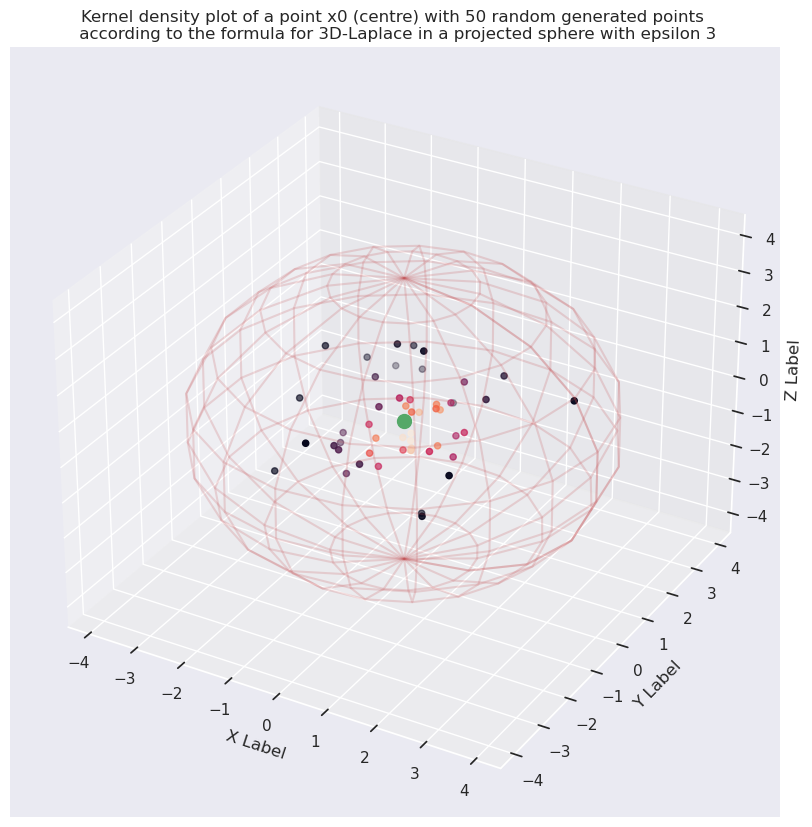
\includegraphics[width=0.6\textwidth]{TheorethicalFramework/ND-Laplace/Images/3d_laplace_noise.png}
  \caption{50 random noise samples generated around point $x_0$ (green dot) using the 3D-Laplace noise method \citep{9646489} plotted on a sphere.}
  \label{fig:3d-laplace-noise}
\end{figure}
Finally, the spherical coordinates are converted to the Cartesian coordinate system to obtain the perturbed location $z$:
\begin{align*}
  z_x = r * \sin(\theta) * \sin(\psi) \\
  z_y = r * \sin(\theta) * \cos(\psi) \\
  z_z = r * \cos(\theta)
\end{align*}
The complete overview is visualized in figure \ref{fig:3d-laplace}.
\begin{figure}
  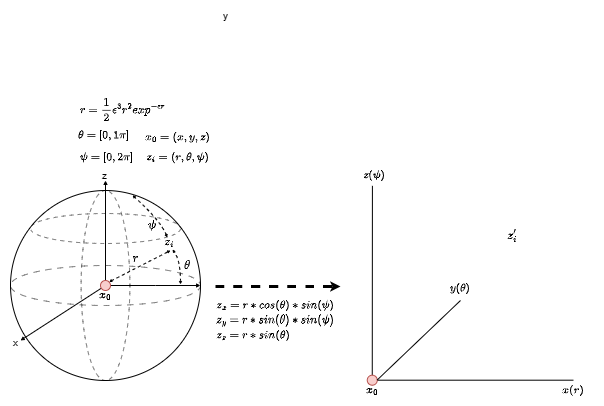
\includegraphics[width=0.8\textwidth]{TheorethicalFramework/ND-Laplace/Images/3d_laplace.png}
  \caption{3D-Laplace noise distribution according to the method proposed by Min et al. \citep{9646489}}
  \label{fig:3d-laplace}
\end{figure}
\newpage
\subsection{Truncation}
As with the 2D-Laplace method, the 3D-Laplace method also needs a truncation method.
This truncation method is also based on the same method as the 2D-Laplace method.
Instead of a plane grid, a cuboid grid is used for 3-dimensional space.
This cuboid remaps the noise to the closest grid cell $g \in G$ or existing point in $X$.
We plotted example data points on a 3-dimensional grid in figure \ref{fig:3d-laplace-example} to demonstrate this:
\begin{figure} [H]
  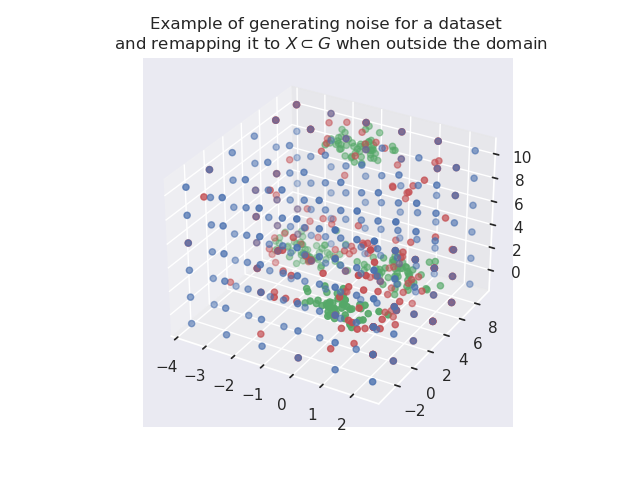
\includegraphics[width=\textwidth]{TheorethicalFramework/ND-Laplace/Images/example_3d_laplace.png}
  \caption{Applying 3-dimensional noise with $\epsilon = 1$ (red dots) to a dataset $X$ (green dots). Demonstrating remapping to the closest grid point (blue) or $X$.}
  \label{fig:3d-laplace-example}
\end{figure}

\newpage
\subsection{Final mechanism}
Finally, we provide as means of a summary the final algorithm for the Laplace mechanism for 3D space
\begin{algorithm}[H]
  \caption{Full algorithm for perturbing training data for 3D-clustering using planar/2D-Laplace \citep{DBLP:journals/corr/abs-1212-1984}}\label{alg:rq1}
  \begin{algorithmic}
    \Require $x \in X$  \Comment 3D array of points
    \Require $l \in R^ +$
    \Require $r \in R^ +$
    \Ensure $z \in Z$ \Comment 3D array of perturbed points
    %\State $r = \frac{\sigma}{2}$ \Comment formula 4.1
    \State $\epsilon \gets \frac{l}{r}$ \Comment Calculating privacy budget \citep{DBLP:journals/corr/abs-1212-1984}
    \State $Z \gets []$
    \For{$point_i \in X$}
    \State $\theta \gets [1, \pi2]$       \Comment Random noise according to equation \ref{eq:3d-laplace-1}.
    \State $p \gets \frac{1}{2\pi}$     \Comment Random noise according to equation \ref{eq:3d-laplace-2}.
    \State $r \gets \frac{1}{2}\epsilon^3 * r^2 * e^{-\epsilon * r}$          \Comment Draw $r$ based on equation \ref{eq:3d-laplace-3}
    %\State $z_i \gets T(x_{min}, x_{max}, point_i, z_i)$ \Comment algorithm 1.
    \State $z_x \gets r * \sin(\theta) * \sin(\psi)$
    \State $z_y \gets r * \sin(\theta) * \cos(\psi)$
    \State $z_z \gets r * \cos(\theta)$
    \State $Z::Add(z)$                      \Comment Adds z to the list Z.
    \EndFor
    \State \Return Z
  \end{algorithmic}
  \label{alg:3d-laplace}
\end{algorithm}
\newpage